\subsection{Original transformations}\label{sub:c3s1s1}
	\paragraph{The original procedures} discussed in \cite{BMUG06} generally work for all sub-classes of \ac{fol}. Those procedures should be applied to a given set of axioms in a specific form called implication form, sometimes it is called a sequent as in here ---ref---, which is explained here -- , and here -- to know how to transform to that form. Moreover, those transformations are guranteed to terminate for any given problem set, which is a gain for us since some of the \ac{epr} problems were not terminating in the original configurations of E.  
%TODO :: to add a reference later

	\subsubsection{What are the Transformations}
	
		\paragraph{} 
		\textbf{The Transformations} are series of procedures, mainly about changing the clauses to certain form named range restricted form. Since the transformations deal with clauses in implication form, then we could define \textbf{Clauses in range restricted form} \ul{to be clauses in which all the variables that appear in the succeedent must exist in the anticedent as well}.
	
		\paragraph{} 
		\textbf{An example for a range restricted clause} is found below:
			\begin{lstlisting}[caption=Range Restricted Clause Example,frame=single,mathescape]			
		
		$ \forall X \forall Y  \left( P(X) \wedge Q(Y) \longrightarrow R(X, Y) \right). $				
		
	where the $\textbf{antecedent}$ here is $ P(X) \wedge Q(Y) $;
	whereas the $\textbf{succeedent}$ is $ R(X, Y) $.
 			\end{lstlisting}
		
		
%TODO :: add the reason later

\begin{comment}		
		\paragraph{} 
		\textbf{For a reason} why this range restricted form will help would be ??
\end{comment}



	 \subsubsection{How do the transformations work}
	 
		\paragraph{} 
		\textbf{Transformations} add a domain predicate to the specification that will help in finding the Model by saying what are the elements of the domain, or the elements of the universe in other words.\par
		Moreover, There are three types of procedures in the transformations:	
		\begin{itemize}
			\item \textbf{Range restricting transformations}
			 \hfill \\ are the first two transformations, and they are the most important type of them. All the rest were added to enhance and improve the range restricting ones. They are responsible for transforming the input clauses to the range restricted form and enumerating the universe/domain of the problem in a way or another. Only one of the two transformations should applied, since they perform the same functionality but in different ways. The two transformations are:
			 	\begin{itemize}
			 		\item \ac{crr}: it enumerates the Herbrand Universe in a naive simple way. 
			 		\item \ac{rr}: it was introduced to improve the naive implementation of the \ac{crr}. So it only adds elements to the domain only when it is needed.
			 	\end{itemize}
			
			\item \textbf{Shifting transformations}
			 \hfill \\ are the second two transformations. They are optional to be used. They complement one another not replace each other. They were introduced mainly to prevent the non-termination of the transformations and to prevent generating and redundant and unpleasant clauses from the steps in \ac{rr} as well. And the two shifting transformations are:
			 	\begin{itemize}
			 		\item \ac{bs}
			 		\item \ac{pf}
			 	\end{itemize}
			
			\item \textbf{\ac{bl}}
			 \hfill \\ is the last transformation and it is optional as well. And It was introduced to detect periodicity that may occur because of function terms. 
		\end{itemize}
		
		\paragraph{} \textbf{Their order of application} is:
			\begin{enumerate}
				\item One of the two range restricting \ac{crr} or \ac{rr}
				\item The Partial Flattening \ac{pf}
				\item The Basic Shifting \ac{bs}
				\item The Blocking \ac{bl} 
			\end{enumerate}			 
		Where the output of a lower number transformation is the input to the higher one. A Flow Chart that summarizes what was explained will be found in Figure ~\ref{fig:original_transformations_flow}.
		
		\begin{figure}[H]
			\centering
 		 	\scalebox{0.38}
 			{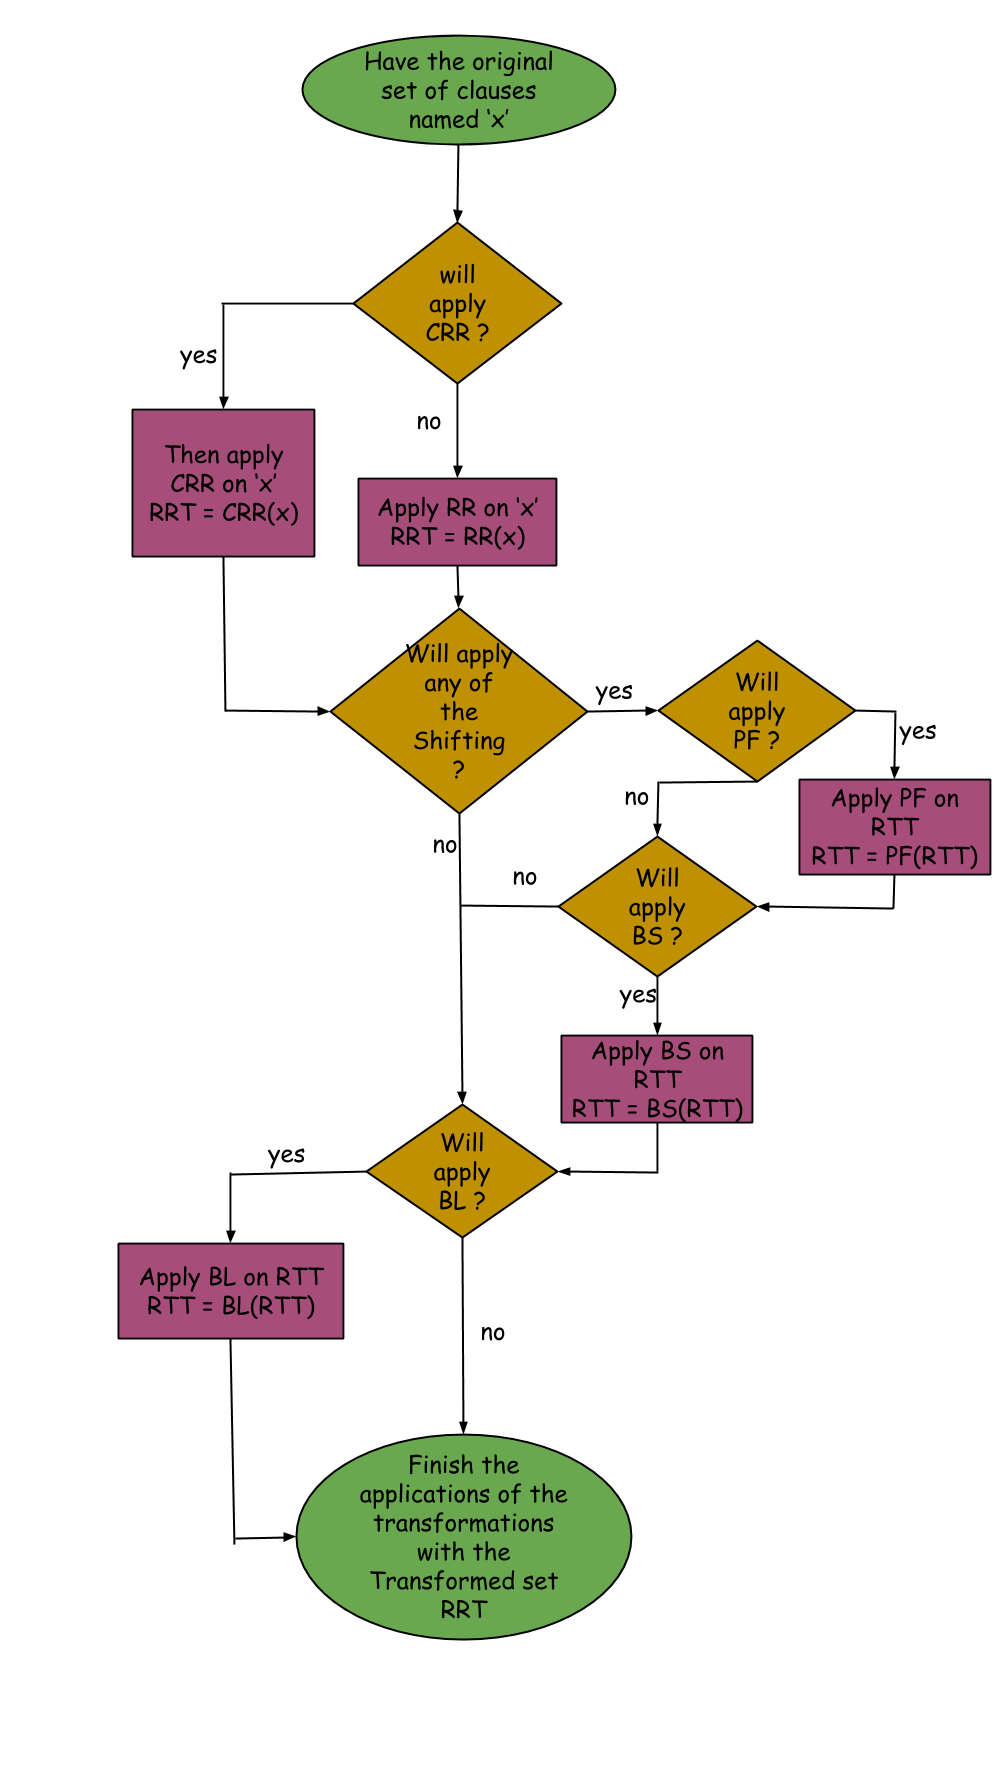
\includegraphics{pictures/Original_transformations_flow.png}}
 			\caption{Flow of the original transformations}\label{fig:original_transformations_flow}
		\end{figure}